\documentclass[a4paper, 11pt]{article}
\usepackage[polish]{babel}
\usepackage[T1]{fontenc}
\usepackage[utf8]{inputenc}
\usepackage{hyperref}
\usepackage{array}
\usepackage{amssymb}
\usepackage{amsmath}
\hypersetup{
    colorlinks,
    citecolor=black,
    filecolor=black,
    linkcolor=black,
    urlcolor=black
}
\usepackage{graphicx}

\usepackage{tikz}
\usetikzlibrary{fit,arrows,matrix,positioning, calc, shapes.gates.logic.IEC, shapes.gates.logic.US}
\tikzstyle{branch}=[fill,shape=circle,minimum size=3pt,inner sep=0pt]

\title{%
        \vspace{-3.5cm}
       \large Sprawozdanie Laboratorium PTC \\
       \huge Realizacja układów kombinacyjnych z wykorzystaniem multipleksera i
pamięci ROM. Układy arytmetyczne.}

\author{Stanisław Fiedler 160250}
\date{LAB 2, 21 października 2024}

\begin{document}

\maketitle
%\tableofcontents

\section{Zadanie 2}\label{sec:zadanie2_} % (fold)

Transkoder wyposażony jest w 4 wejścia i 4 wyjścia.
Jego działanie przedstawiono w Tabeli 1.
Wszystkie wartości zakodowane w naturalnym kodzie binarnym (NBC).
Wybierz kolumnę odpowiadającą ostatniej cyfrze Twojego numeru indeksu.
Zrealizuj transkoder korzystając z programu Logisim z użyciem pamięci ROM i wypróbuj jego działanie.

\begin{center}
	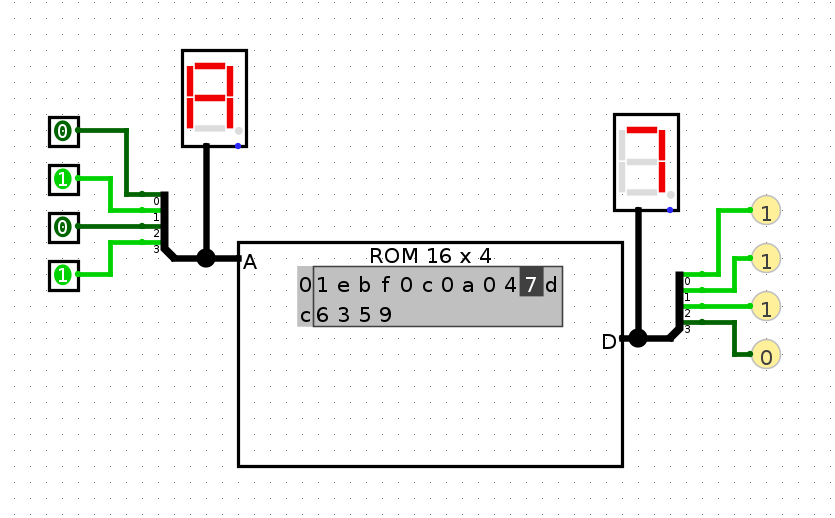
\includegraphics[scale=0.4]{images/Pasted image.png}
\end{center}

% section Zadanie 2 (end)

\section{Zadanie 4d}\label{sec:zadanie4_} % (fold)
Sumator wielobitowy można zrealizować jako układ iteracyjny zbudowany z łańcucha połączonych sumatorów 1-bitowych.
Czy na podobnej zasadzie można zrealizować układ realizujący odejmowanie?
Jak będą wyglądały funkcje różnica i pożyczka?

\begin{center}

	\begin{tabular}{ | c | c | c || c | c | }
		\hline
		a & b & c & różnica & pożyczka \\
		\hline\hline
		0 & 0 & 0 & 0       & 0        \\
		0 & 0 & 1 & 1       & 1        \\
		0 & 1 & 0 & 1       & 1        \\
		0 & 1 & 1 & 0       & 1        \\
		1 & 0 & 0 & 1       & 0        \\
		1 & 0 & 1 & 0       & 0        \\
		1 & 1 & 0 & 0       & 0        \\
		1 & 1 & 1 & 1       & 1        \\
		\hline
	\end{tabular}

\end{center}

\vspace{0.5cm}

\begin{center}
	\Large Różnica\\
	\begin{tikzpicture}
		\matrix (Y1) [matrix of math nodes, nodes in empty cells, nodes={minimum height=1cm, minimum width=1cm, anchor=center}, column 1/.style={nodes={minimum height=1cm, minimum width=2cm, anchor=center}}] (m)
		{
				{} & 00 & 01 & 11 & 10 \\
				0             & 0  & 1  & 0  & 1  \\
				1             & 1  & 0  & 1  & 0  \\
			};
		\draw[double distance=2pt] (m-1-2.north west) -- (m-3-2.south west);
		\draw[double distance=2pt] (m-1-1.south west) -- (m-1-5.south east);;
		\node[fit={(m-2-3.north west) (m-2-3.south east)},
			thick, inner sep=0pt, rounded corners=1mm,
			draw=green ]{};
		\node[fit={(m-2-5.north west) (m-2-5.south east)},
			thick, inner sep=0pt, rounded corners=1mm,
			draw=blue ]{};
		\node[fit={(m-3-2.north west) (m-3-2.south east)},
			thick, inner sep=0pt, rounded corners=1mm,
			draw=red ]{};
		\node[fit={(m-3-4.north west) (m-3-4.south east)},
			thick, inner sep=0pt, rounded corners=1mm,
			draw=orange ]{};
		\draw (m-1-1.north west) -- (m-1-1.south east);
		\node[anchor=south west, font=\Large] at (m-1-1.center) {$bc$};
		\node[anchor=north east, font=\Large] at ($(m-1-1.center) + (-0.2,0.1)$) {$a$};
	\end{tikzpicture}

	\Large $ \quad R = a\bar{b}\bar{c} + \bar{a}\bar{b}c + abc + \bar{a}b\bar{c} $
\end{center}

\vspace{0.5cm}

\begin{center}
	\Large Pożyczka\\
	\begin{tikzpicture}
		\matrix (Y1) [matrix of math nodes, nodes in empty cells, nodes={minimum height=1cm, minimum width=1cm, anchor=center}, column 1/.style={nodes={minimum height=1cm, minimum width=2cm, anchor=center}}] (m)
		{
				{} & 00 & 01 & 11 & 10 \\
				0             & 0  & 1  & 1  & 1  \\
				1             & 0  & 0  & 1  & 0  \\
			};
		\draw[double distance=2pt] (m-1-2.north west) -- (m-3-2.south west);
		\draw[double distance=2pt] (m-1-1.south west) -- (m-1-5.south east);;
		\node[fit={(m-2-3.north west) (m-2-4.south east)},
			thick, inner sep=0pt, rounded corners=1mm,
			draw=green ]{};
		\node[fit={(m-2-4.north west) (m-2-5.south east)},
			thick, inner sep=0pt, rounded corners=1mm,
			draw=blue ]{};
		\node[fit={(m-2-4.north west) (m-3-4.south east)},
			thick, inner sep=0pt, rounded corners=1mm,
			draw=red ]{};
		\draw (m-1-1.north west) -- (m-1-1.south east);
		\node[anchor=south west, font=\Large] at (m-1-1.center) {$bc$};
		\node[anchor=north east, font=\Large] at ($(m-1-1.center) + (-0.2,0.1)$) {$a$};
	\end{tikzpicture}
	\raisebox{1cm}{\Large $ \quad P = bc + \bar{a}c + \bar{a}b $}
\end{center}

\vspace{0.5cm}

\begin{center}
	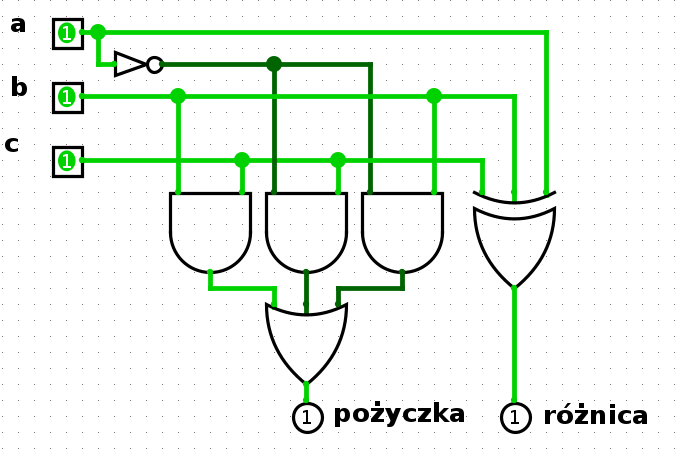
\includegraphics[scale=0.3]{images/Pasted image (2).png}
\end{center}

% section Zadanie 4d (end)

\section{Zadanie 7}\label{sec:zadanie7_} % (fold)
Przedstaw oczekiwane wyniki przedstawionego niżej programu. Następnie wykonaj program i porównaj wyniki.

Program żeby poprawnie przypisać wartość zmiennej o mniejszym rozmiarze do zmiennej o większej liczbie bitów musi odpowiednio uzupełnić najstarsze bity nowej zmiennej aby zachować oryginalny moduł. W przypadku liczb ujemnych powinno to być 1, a dodatnich 0.

Program przypisuje wartość 000F do zmiennej ze znakiem (sa) i bez (usa).
W obu przypadkach jest interpretowana jako dodatnia więc na miejsca najstarszych bitów wstawiane są 0.
Wartość FFFB przypisana do zmiennych usb i sb jest interpretowana różnie.
Zmienna ze znakiem uznaje ją za wartość ujemną więc, aby zachować znak, podczas rozszerzania dopisywane są 1. Zmienna bez znaku interpretuje ją jako dodatnią więc z przodu dopisywane są 1.


% section Zadanie 7 (end)

\section{Zadanie 8}\label{sec:zadanie8_} % (fold)
Przedstaw w postaci dwójkowej i szesnastkowej liczby następujące liczby 16-bitowe w kodzie U2.

\[
	\begin{array}{c | c | c | c}
		\text{liczba}      & \text{dwójkowo}       & \text{szesnastkowo} & \text{dziesiętnie} \\
		\hline
		5_{10}             & 0000000000000101_{U2} & 0005                &                    \\
		-5_{10}            & 1111111111111011_{U2} & FFFB                                     \\
		\text{największa}  & 0111111111111111_{U2} & 7FFF                & 32767_{10}         \\
		\text{najmniejsza} & 1000000000000000_{U2} & 8000                & -32768_{10}
	\end{array}
\]

% section Zadanie 8 (end)

\section{Zadanie 9}\label{sec:zadanie_} % (fold)
Wyjaśnij, dlaczego wyniki programu 2 są takie jak pokazano poniżej.

\begin{enumerate}
	\item [a)] $121 \quad 34 \quad 155$ \\
	      155 jest poprawnym wynikiem dodawania.
	\item[b)] 20000 \quad 1000 \quad 21000 \\
	      21000 jest poprawnym wynikiem dodawania.
	\item[c)] 20000 \quad 30000 \quad -15536 \\
	      Do zapisania wyniku dodawania 20000 + 30000 w kodzie U2 potrzeba 17 bitów. Typ short może przechowac tylko 16, liczba reperzentowana przez 16 najmniej znaczączych bitów to -15536.
	\item[d)] -20000 \quad -3000 \quad -23000 \\
	      -23000 jest poprawnym wynikiem odejmowania.
	\item[e)]  -20000 \quad -25000 \quad 20536 \\
	      Do zapisania wyniku odejmowania -20000-25000 w kodzie U2 potrzeba 17 bitów. Typ short może przechowac tylko 16, liczba reperzentowana przez 16 najmniej znaczączych bitów to 20536.

\end{enumerate}

% section Zadanie 9 (end)

\end{document}
